\documentclass[a4paper,10pt]{beamer}

\usepackage[utf8]{inputenc}
\usepackage{fontspec}
\usepackage{amsmath}
\usepackage{amssymb}
\usepackage{graphicx}
\usepackage{subcaption}
\usepackage{comment}
\usepackage{wrapfig}
\usepackage{color}
\usepackage{xcolor}
\usepackage{mathtools}
\usepackage{algorithmicx}
\usepackage{algorithm}
\usepackage{algpseudocode}
\usepackage{hyperref}
\usepackage{cleveref}
\usepackage{empheq}
\usepackage{mathrsfs,euscript}
\usepackage{tcolorbox}

\beamertemplatenavigationsymbolsempty

\bibliographystyle{unsrt}

\usefonttheme{professionalfonts}

\usefonttheme[]{structurebold}

\usetheme{Copenhagen}
\usecolortheme{rose}
\usecolortheme{dolphin}
\useinnertheme{circles}
\useoutertheme{tree}

\addtobeamertemplate{navigation symbols}{}{%
	\usebeamerfont{footline}%
	\usebeamercolor[fg]{footline}%
	\hspace{1em}%
	\insertframenumber/\inserttotalframenumber
}

\setbeamertemplate{headline}{%
	\leavevmode%
	\hbox{%
		\begin{beamercolorbox}[wd=\paperwidth,ht=2.5ex,dp=1.125ex]{palette quaternary}%
		\end{beamercolorbox}%
	}
}

\setmainfont[Path=/usr/share/fonts/truetype/calibri/,
BoldItalicFont=calibriz.ttf,
BoldFont      =calibrib.ttf,
ItalicFont    =calibrii.ttf]{calibri.ttf}

\newcommand{\BS}[1]{\boldsymbol{#1}}
\newcommand{\E}[1]{\mathbb{E}\left[ #1 \right]}
\newcommand{\sqb}[1]{\left[ #1 \right]}
\newcommand{\rb}[1]{\left( #1 \right)}
\newcommand{\cb}[1]{\left \{ #1 \right \}}
\newcommand{\angbrac}[1]{\left \langle #1 \right \rangle}
\newcommand{\norm}[1]{\left| \left| #1 \right| \right|}

\definecolor{burgundy}{RGB}{128,0,32}
\definecolor{darkgreen}{RGB}{4,110,0}

\definecolor{customblue}{rgb}{0.8,0.8,1}
\newcommand*\bluebox[1]{\colorbox{customblue}{\hspace{1em}#1\hspace{1em}}}

\definecolor{custompurple}{RGB}{255,179,179}
\newcommand*\purplebox[1]{\colorbox{custompurple}{\hspace{1em}#1\hspace{1em}}}

\title{Generalized Langevin Equation}
\subtitle{Stochastic Differential Equations}
\author{Sankarasubramanian Ragunathan \newline \newline 389851}
\institute{\textbf{RWTH Aachen University}}
\date{}


\begin{document}
	\begin{frame}
		\titlepage
		\centering
		
\includegraphics[width=0.25\textwidth]{RWTH_Aachen_University_Logo.eps}
	\end{frame}

	\begin{frame}
	\frametitle{Agenda}
		\footnotesize
		\tableofcontents
	\end{frame}

	\begin{frame}
		\normalsize
		\section{Scope of the Project}
		\frametitle{Scope of the Project}
		
		\begin{itemize}
			\item[What?]{Generalized Langevin Dynamics is a modeling technique that can be used to model anomalous diffusive phenomena observed in viscoelastic fluids.}
			
			\item[Why?]{GLE succeeds in capturing sub-diffusive and super-diffusive behavior. But GLE is \textit{Non-Markovian} i.e. \texttt{memory kernel} depends on the history of velocity. This issue is overcome by using Extended Variable GLE that considers a finite dimensional subspace for the \texttt{memory kernel}.}
			
			\item[How?]{Study Extended Variable GLE using Prony series approximation. Accuracy of Explicit Euler and Splitting Numerical schemes are also tested to find out the "optimal scheme". Study local and global sensitivity of the observables to perturbations of the extended variable GLE.}
			
			\item[Where?]{Applications of GLE include but are not restricted to micro-rheology, biological systems, nuclear quantum effects and systems in which anomalous diffusion arise.}
			
		\end{itemize}
	\end{frame}

	\begin{frame}
		\small
		\section{Introduction to Generalized Langevin Equation}
		\subsection{Langevin dynamics as a computational tool}
		\frametitle{Langevin dynamics as a computational tool}
		\begin{itemize}
			\item[What?] {\textbf{Langevin Dynamics:} Large particles in a bath of small particles, motion of large particles directly integrated while the dynamics of small particles are "averaged out".}
			\item[Why?] {\textit{Molecular Dynamics} simulations involving all particles is computationally expensive. Langevin Equation model is computationally cheaper.}
		\end{itemize}
		\begin{minipage}{0.35\linewidth}
			\footnotesize
			\begin{alertblock}{Drawback}
				Anomalous diffusion problems arising due to \textit{Power Law} behavior of solute-solvent systems cannot be solved.
			\end{alertblock}
			\begin{exampleblock}{Solution}
				\textit{Generalized Langevin Equation} (\textbf{GLE})
			\end{exampleblock}
		\end{minipage}
		\hfill
		\begin{minipage}{0.6\linewidth}
			\centering
			\begin{figure}[H]
				\begin{subfigure}[b]{0.45\linewidth}
					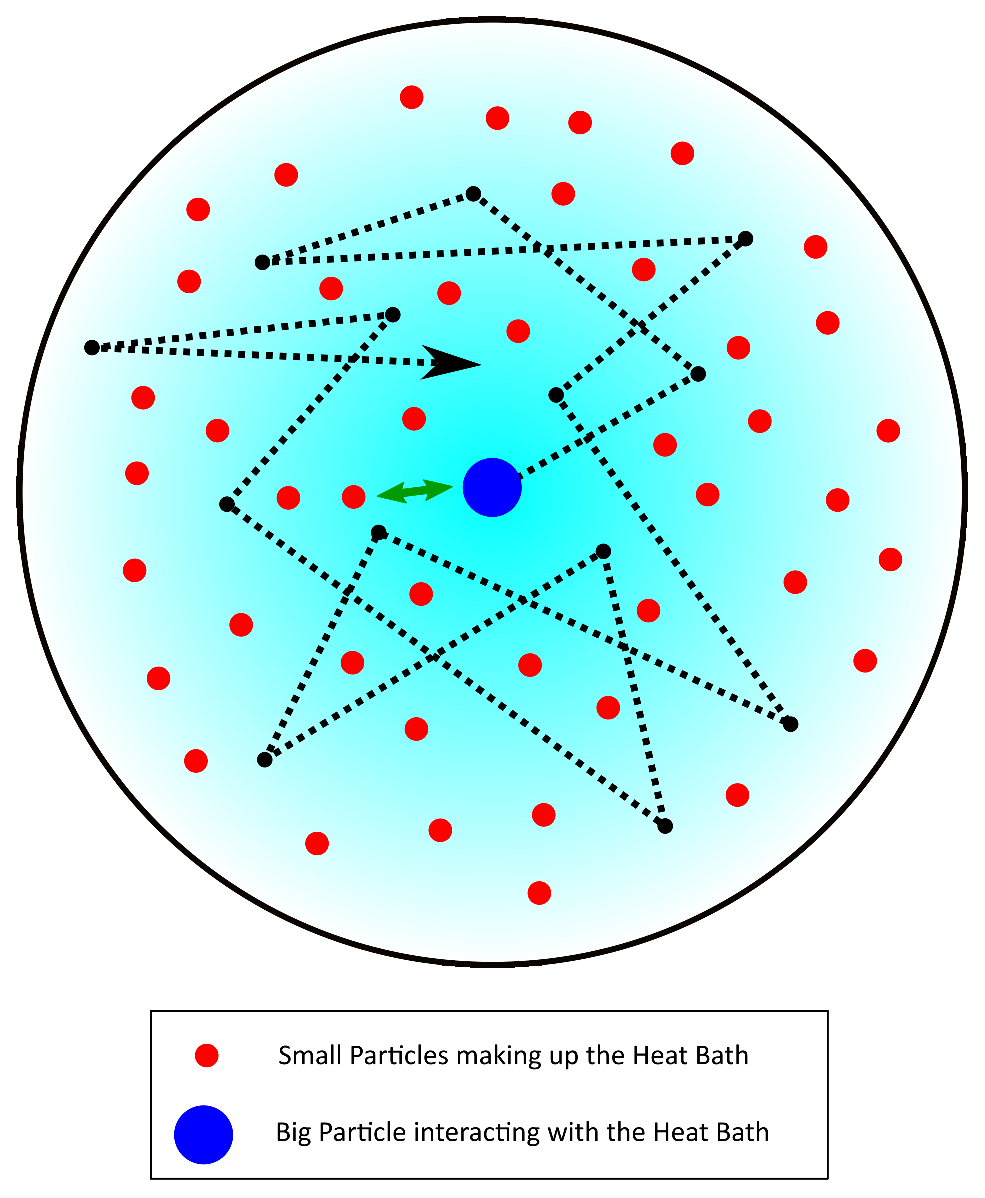
\includegraphics[width=\linewidth]{./Plots/HeatBath.eps}
					\caption{\footnotesize \textcolor{blue}{Big Particles} interacting with \textcolor{red}{Smaller Particles}}
				\end{subfigure}
				\begin{subfigure}[b]{0.5\linewidth}
					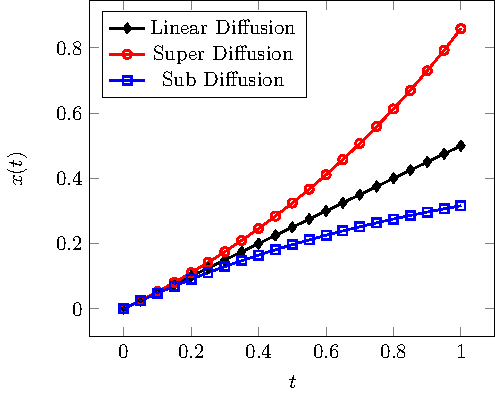
\includegraphics[width=\linewidth]{./Plots/Diffusion.pdf}
					\caption{\footnotesize Sub-diffusive and Super-diffusive behavior of solute-solvent systems}
				\end{subfigure}
			\end{figure}
		\end{minipage}
	\end{frame}		
	
	\begin{frame}
		\small
		\subsection{Stochastic systems with memory capture for anomalous diffusion}
		\frametitle{Mathematical Model for Anomalous Diffusion}
		
		The velocity term of GLE is based on \textit{Ornstein-Uhlenbeck} process.
	
		\begin{block}{GLE Equations}
			\begin{align}
			d\BS{X}(t) &= \BS{V}(t) dt \\
			\BS{M} d\BS{V}(t) &= \underbrace{\vphantom{- \int_{0}^{t} \BS{\Gamma}(t-s) \BS{V}(s) ds dt}\BS{F}^{c}(\BS{X}(t)) dt}_{\text{\centering \begin{minipage}{1.5cm}
					Conservative Force due to Potential
			\end{minipage}}}
			\underbrace{- \int_{0}^{t} \BS{\Gamma}(t-s) \BS{V}(s) ds dt}_{\text{\centering \begin{minipage}{1.5cm}
				Temporally Non-Local Drag Force
				\end{minipage}}\;\rb{\BS{F}^{d}}} + \underbrace{\vphantom{- \int_{0}^{t} \BS{\Gamma}(t-s) \BS{V}(s) ds dt}\BS{F}^{r}(t)dt}_{\text{\begin{minipage}{1.8cm}
				Random Correlated Force given by \textit{FDT}
				\end{minipage}}} \\
			\BS{X}(0) = \BS{X}_{0}, &\qquad \BS{V}(0) = \BS{V}_{0} \qquad (\text{Initial Conditions})
			\end{align}
		\end{block}
		\begin{alertblock}{Note:}
			$\BS{F}^{r}$ and $\BS{F}^{d}$ are characterized by the \texttt{memory kernel} consistent with \textbf{FDT}.
		\end{alertblock}
	\end{frame}

	\begin{frame}
		\small
		\frametitle{Mathematical Model for Anomalous Diffusion}
		\begin{theorem}
			FDT (Fluctuation Dissipation Theorem) states that the equilibration to a temperature, $T$, requires that the two-time correlation of $\BS{F}^{r}(t)$ and $\BS{\Gamma}(t)$ be related as:
			\begin{align}
				\angbrac{\BS{F}^{r}_{i}(t+s),\BS{F}^{r}_{j}(t)} = \text{k}_{\text{B}} T \BS{\Gamma}(s) \delta_{ij}, \qquad s \geq 0
			\end{align}
		\end{theorem}
		where $\text{k}_{\text{B}}$ is the Boltzmann's Constant, $\delta_{ij}$ is the Kronecker Delta and $i$,$j$ represent distinguished non-interacting particles (in our case, the solute particles that we are modeling). Hence FDT correlates the random forces for a given solute particle at different times.
		\linebreak
		
		
		\textcolor{red}{\textbf{Note:}}
		\begin{itemize}
			\item {$\BS{F}^{d}(t)$ depends on the velocity history unlike in \textit{Langevin Equation}} where it depends on the velocity at that instant.
			\item {The random forces are not just delta correlated but are correlated by the \texttt{memory kernel}. \textcolor{darkgreen}{\texttt{Memory Kernel} choice and approximation important based on the problem to be studied.}}
		\end{itemize}
	\end{frame}
	
	\begin{frame}
		\subsection{Complications due to memory effects}
		\frametitle{Complications due to memory effects}
		\vspace{-0.8cm}
		\begin{minipage}[t]{0.44\textwidth}
			\begin{alertblock}{\textbf{Complications}}
				\begin{enumerate}
					\item {Storage of subset of the time history of $\BS{V}(t)$.}
					\item {Sequence of $\BS{F}^{r}(t)$ given by \texttt{FDT}.}
					\item {Numerical SDE solution should converge in distribution.}
				\end{enumerate}
			\end{alertblock}
		\end{minipage}
		\hfill
		\begin{minipage}[t]{0.52\textwidth}
			\centering
			\begin{exampleblock}{\textbf{Solution}}
				\begin{enumerate}
					\item {Using extended variable \texttt{Prony Series} for \texttt{Memory Kernel}.
					\scriptsize
					\begin{align}
					 \BS{\Gamma}(t) \approx \sum_{k=1}^{N_{k}} \frac{c_{k}}{\tau_{k}} \exp \sqb{-\frac{t}{\tau_{k}}}, \qquad t \geq 0 \end{align}
					\normalsize
					where $N_{k}$ is the number of terms used in approximating the \texttt{memory kernel}. }
					\item {Using a suitable integration scheme for the numerical method.}
				\end{enumerate}
			\end{exampleblock}
		\end{minipage}
	\end{frame}

	\begin{frame}
		\frametitle{Complications due to memory effects}
		\small
		\textcolor{blue}{\textbf{Why use extended variable Prony Series?}}
		
		\begin{itemize}
			\item {Approximation of \texttt{memory kernel} to map {\textbf{Non-Markovian}} GLE to {\textbf{Markovian}} system of $N_{k}$ variables.}
			\item {Typically used for modelling \textit{Power Law} based decay/growth as observed in sub/super diffusive systems.}
		\end{itemize}
		
		\textcolor{blue}{\textbf{Importance of choice of integration scheme?}}
		
		\begin{itemize}
			\item {Conservation of moments of variables of interest such as displacement and velocity (usual variables of interest for MD simulations)}
			\item {Convergence of \textbf{GLE} to Langevin equation in the limit of small $\tau_{k}$ as observed in theory.}
		\end{itemize}
	
		\textcolor{red}{\textbf{Note:}} In the numerical experiments carried out in this presentation, we consider sub-diffusive decaying behavior which behaves as $t^{-\alpha}$ where $\alpha < 1$ and hence we use a decaying Prony series to approximate the memory function.
	\end{frame}

	\begin{frame}
		\subsection{Extended Variable GLE formulation}
		\frametitle{Extended Variable GLE formulation}
		\vspace{-0.3cm}
 		%\textbf{Extended Variable GLE:}
		\tiny
		\begin{block}{Main Extended Variable GLE Equations}
			\vspace{-0.3cm}
			\begin{flalign}
				m_{i} dV_{i}(t) &=  F_{i}^{c}(\BS{X}(t))dt + \sum_{k=1}^{N_{k}} S_{i,k} dt \\
				dX_{i}(t) &= V_{i}(t)dt\\
				dS_{i,k}(t) &= -\frac{1}{\tau_{k}}S_{i,k}(t)dt-\frac{c_{k}}{\tau_{k}}V_{i}(t) dt + \frac{1}{\tau_{k}}\sqrt{2 \text{k}_{\text{B}} T c_{k}} dW_{i,k}(t)
			\end{flalign}
		\end{block}
		\begin{block}{Auxiliary Extended Variable GLE Equations}
			\vspace{-0.3cm}
			\begin{flalign}
				S_{i,k}(t) &= Z_{i,k}(t) + F_{i,k}(t) \\
				dZ_{i,k}(t) &= -\frac{1}{\tau_{k}} Z_{i,k}(t)dt - \frac{c_{k}}{\tau_{k}}V_{i}(t)dt &&
				Z_{i,k}(t) = -\int_{0}^{t} \frac{c_{k}}{\tau_{k}} \text{exp} \sqb{-\frac{\rb{t-s}}{\tau_{k}}}V_{i}(s)ds \\
				d F_{i, k}(t)&=-\frac{1}{\tau_{k}} F_{i, k}(t) d t +\frac{1}{\tau_{k}} \sqrt{2 {k}_{B} T c_{k}} d W_{i, k}(t) && \angbrac{F_{i,k}(t+s),F_{i,k}(t)} = \text{k}_{\text{B}}T\frac{c_{k}}{\tau_{k}} \text{exp}\sqb{-\frac{s}{\tau_{k}}} \\
				&\quad && F_{i}^{r}(t) = \sum_{k=1}^{N_{k}} F_{i,k}(t)
			\end{flalign}
		\end{block}
	\end{frame}
	
	\begin{frame}
		\section{Numerical Schemes}
		\subsection{Explicit Euler vs. Splitting Schemes}
		\frametitle{Explicit Euler vs. Splitting Schemes}
		\footnotesize
		\textcolor{blue}{\textbf{Numerical Schemes:}}
		\begin{itemize}
			\item {Explicit Euler Scheme.}
			\item {Splitting Scheme.}
		\end{itemize}
		\begin{alertblock}{Which numerical scheme to choose for solving the problem?}
			General observables/physical quantities that are measured to understand the behavior of a system. E.g., \textit{Mean Square Displacement} (\texttt{MSD}) and \textit{Velocity Autocorrelation Function} \texttt{VAF} in microrheology. Therefore essential to consider scheme that conserves the first and second moments of $\BS{V}(t)$ and $\BS{X}(t)$ for validating the simulations.
		\end{alertblock}
		\textcolor{blue}{\textbf{Implementation Details:}}
		\begin{itemize}
			\item {Uniform time-step size, $\Delta t$, where $N_{t} \Delta t = T_{\text{tot}}$ ($T_{\text{tot}}$ represents the total time of the simulation and $N_{t}$ represents the \# of time-steps.)}
			\item {All $N_{p}$ particles are seeded with the same constant $\BS{X}(0)$ and $\BS{V}(0)$ (\textcolor{red}{\textbf{Note:}} We could also seed the initial conditions based on \textit{Boltzmann} distribution.)}
			\item {The composite variable $S_{i,k}(t)$ is assumed to be zero initially.}
		\end{itemize}
	\end{frame}
	
	\begin{frame}
		\frametitle{Explicit Euler vs. Splitting Schemes}
			\vspace{-0.3cm}
			\begin{algorithm}[H]
				\scriptsize
				\renewcommand{\algorithmicrequire}{\textbf{Input:}}
				\renewcommand{\algorithmicensure}{\textbf{Output:}}
				\begin{algorithmic}[1]
					\Require $\BS{X}(0)$,$\BS{V}(0)$,$\BS{S}(0)$
					\Ensure $\BS{X}(t)$,$\BS{V}(t)$
					\For{$n=0$ to $N_{t}$}
					\tiny
						\State $V_{i}^{n+1} = V_{i}^{n} + \frac{\Delta t}{m_{i}} F_{i}^{c} \rb{\BS{X}^{n}}+\frac{\Delta t}{m_{i}} \sum_{k=1}^{N_{k}}S_{i,k}^{n}$
						\Comment Advance $\BS{V}(t)$ by a full step
						\State $X_{i}^{n+1} = X_{i}^{n} + \Delta t V_{i}^{n}$
						\Comment Advance $\BS{X}(t)$ by a full step
						\State $S_{i,k}^{n+1} = \rb{1-\frac{\Delta t}{\tau_{k}}}S_{i,k}^{n}-\frac{c_{k}\Delta t}{\tau_{k}}V_{i}^{n} + \frac{1}{\tau_{k}}\sqrt{2 \text{k}_{\text{B}} T c_{k}}\Delta W_{i,k}$
						\Comment Advance $\BS{S}(t)$ by a full step
					\scriptsize
					\EndFor
				\end{algorithmic}
				\caption*{Explicit Euler Scheme}
			\end{algorithm}
			\vspace{-0.75cm}
			\begin{algorithm}[H]
				\scriptsize
				\renewcommand{\algorithmicrequire}{\textbf{Input:}}
				\renewcommand{\algorithmicensure}{\textbf{Output:}}
				\begin{algorithmic}[1]
					\Require $\BS{X}(0)$,$\BS{V}(0)$,$\BS{S}(0)$
					\Ensure $\BS{X}(t)$,$\BS{V}(t)$
					\For{$n=0$ to $N_{t}$}
					\tiny
					\State $V_{i}^{n+1/2} = V_{i}^{n} + \frac{\Delta t}{2m_{i}} F_{i}^{c} \rb{\BS{X}^{n}}+\frac{\Delta t}{2m_{i}} \sum_{k=1}^{N_{k}}S_{i,k}^{n}$
					\Comment Advance $\BS{V}(t)$ by a half step
					\State $X_{i}^{n+1} = X_{i}^{n} + \Delta t V_{i}^{n+1/2}$
					\Comment Advance $\BS{X}(t)$ by a full step
					\State $S_{i,k}^{n+1} = \theta_{k} S_{i,k}^{n}-\rb{1-\theta_{k}}c_{k}V_{i}^{n+1/2} + \alpha_{k}\sqrt{2 \text{k}_{\text{B}} T c_{k}}\Delta W_{i,k}$
					\Comment Advance $\BS{S}(t)$ by a full step
					\State $V_{i}^{n+1} = V_{i}^{n+1/2} + \frac{\Delta t}{2m_{i}} F_{i}^{c} \rb{\BS{X}^{n+1}}+\frac{\Delta t}{2m_{i}} \sum_{k=1}^{N_{k}}S_{i,k}^{n+1}$
					\Comment Advance $\BS{V}(t)$ by a half step
					\scriptsize
					\EndFor
				\end{algorithmic}
				\caption*{Splitting Scheme}
			\end{algorithm}
	\end{frame}

	\begin{frame}
		\frametitle{Explicit Euler vs. Splitting Schemes - Case Study}
		\textcolor{blue}{\textbf{Assumptions:}}
		\begin{itemize}
			\item {One dimensional problem, $d = 1$}
			\item {Single mode in the Prony series approximation, $N_{k} = 1$}
			\item {Zero conservative force acting on the particles, $\BS{F}^{c}\rb{\BS{X}(t)} = 0$}
		\end{itemize}
		The case study is simulated using both numerical schemes, \textit{Explicit Euler} and \textit{Splitting Method}, for three different $\tau$ and $c$ values in the \texttt{Prony Series} approximation (\Cref{tab:cTauBaseCase})
		\begin{table}[H]
			\begin{tabular}{| p{2.6cm} | c | c |}
				\hline
				\textbf{Type of System} & $\BS{c}$ & $\BS{\tau}$ \\
				\hline
				Under-damped & 1 & 1 \\
				Critically-damped & 0.5 & 0.5 \\
				Over-damped & 0.25 & 0.25 \\
				\hline
			\end{tabular}
			\caption{$c$ and $\tau$ values used for the case study}
			\label{tab:cTauBaseCase}
		\end{table}
	\end{frame}

	\begin{frame}
		\subsection{First and Second moment conserving Splitting schemes}
		\footnotesize
		\frametitle{Explicit Euler vs. Splitting Schemes - Results}
		\begin{figure}[H]
			\centering
			\begin{subfigure}[b]{0.326\linewidth}
				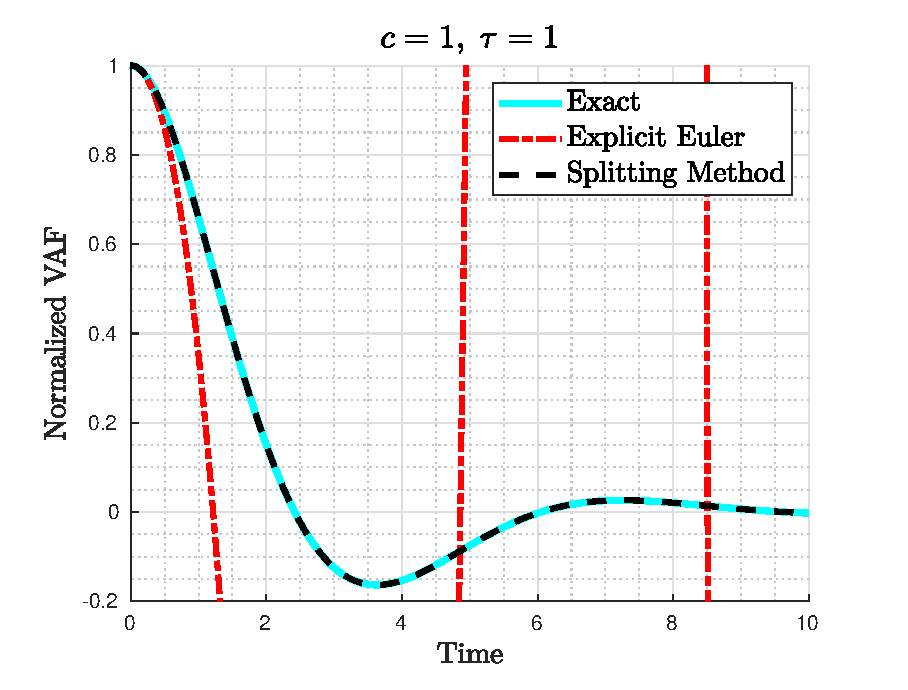
\includegraphics[width=\linewidth]{./Plots/CaseStudy/nonnorm_scale_under.eps}
				\caption{Under-damped}
			\end{subfigure}
			\begin{subfigure}[b]{0.326\linewidth}
				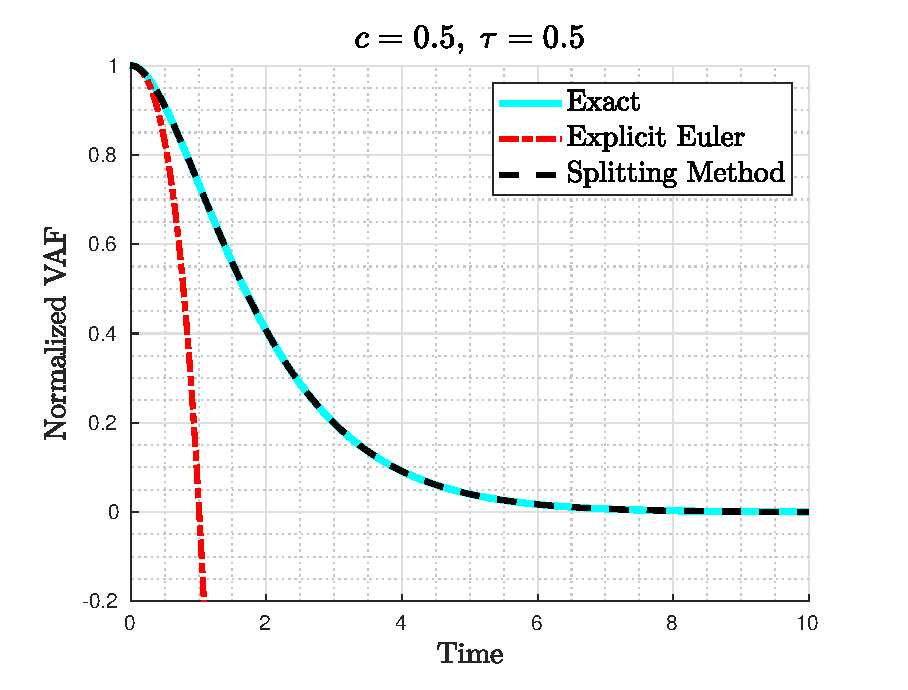
\includegraphics[width=\linewidth]{./Plots/CaseStudy/nonnorm_scale_critical.eps}
				\caption{Critically-damped}
			\end{subfigure}
			\begin{subfigure}[b]{0.326\linewidth}
				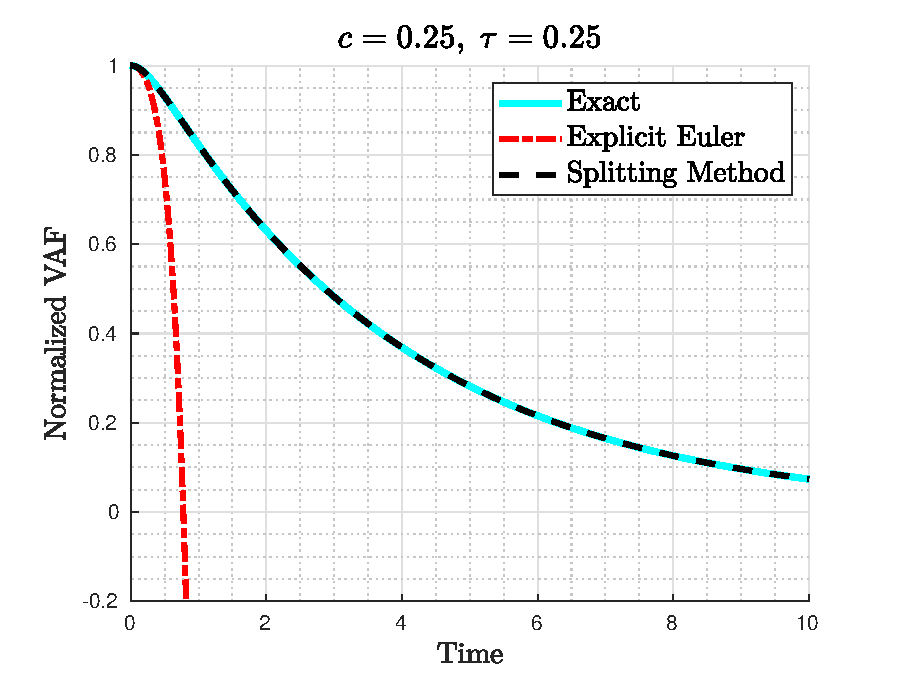
\includegraphics[width=\linewidth]{./Plots/CaseStudy/nonnorm_scale_over.eps}
				\caption{Over-damped}
			\end{subfigure}
			\caption{Normalized VAF vs. Time for Explicit Euler and Splitting schemes($\delta t = 0.01, N_{p} = 1000, N_{k} = 1$)}
		\end{figure}
		\vspace{-0.5cm}
		\begin{alertblock}{Normalized VAF (\textit{Velocity Autocorrelation Function})}
			\begin{align}
				\frac{\angbrac{\BS{V}(t),\BS{V}(0)}}{\angbrac{\BS{V}(0),\BS{V}(0)}} = 
				\begin{cases}
				\text{exp} \sqb{-\frac{t}{2 \tau}} \rb{\cos\rb{\Omega t} + \frac{1}{2\tau\Omega} \sin\rb{\Omega t}}  &\text{for} \; \Omega \neq 0 \\
				\text{exp} \sqb{-\frac{t}{2 \tau}} \rb{1 + \frac{t}{2 \tau}} &\text{for} \; \Omega = 0
				\end{cases}
				\label{eq:oneModeExactVAF}
			\end{align}
			\begin{gather}
				\notag
				\Omega = \sqrt{c/\tau - 1/4\tau^{2}}
			\end{gather}
			\textbf{Note:} One mode Prony series approx. without any conservative force terms.
		\end{alertblock}
	\end{frame}

	\begin{frame}
		\frametitle{Explicit Euler vs. Splitting Schemes - Results}
		\begin{figure}[H]
			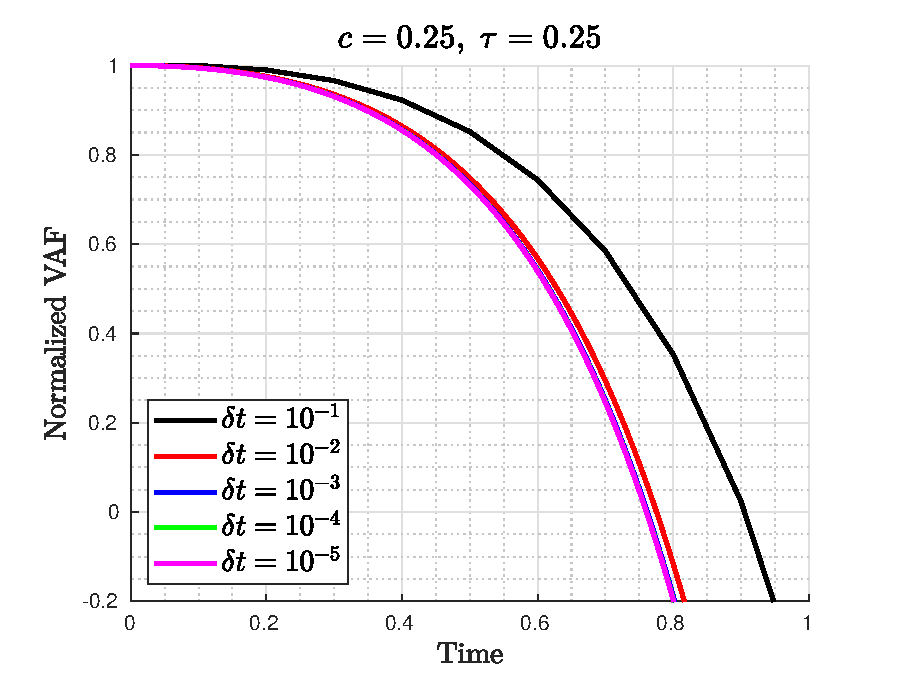
\includegraphics[width=0.75\linewidth]{./Plots/timeStepVariation/timeVariation.eps}
			\caption{\footnotesize Normalized VAF vs. Time for Explicit Euler scheme for different time step sizes. Here we have considered zero conservative force acting on the particles with one mode Prony series approximation. We can see that even on using very fine time-step size, the Explicit Euler scheme does not conserve moments.}
		\end{figure}
	\end{frame}
	
	\begin{frame}
		\frametitle{\large First and Second moment conserving Splitting schemes}
		\large
		\textcolor{blue}{\textbf{Observation:}}
		{Explicit Euler scheme produces wrong results for the \texttt{Normalized VAF} as when compared to the Splitting scheme} (\textit{\textbf{Reason:} Independent updates for $\BS{X}(t)$ and $\BS{V}(t)$ when using Explicit Euler scheme.}) \\
		\vspace{0.25cm}
		\textcolor{blue}{\textbf{Solution:}}
		{Using the Splitting scheme as the preferred integration scheme for all proceeding numerical experiments and sensitivity analysis studies.}
	\end{frame}
	
	\begin{frame}
		\subsection{Numerical experiments - Splitting scheme applied to Harmonic Potential Well}
		\frametitle{Harmonic Potential Well - Problem}
		\begin{block}{Harmonic Potential Well GLE}
			\footnotesize
			\begin{align}
				d\BS{V}(t) = \underbrace{\vphantom{\int_{0}^{t} \frac{\gamma_{\lambda}}{\Gamma_{0} \rb{1-\lambda}}\rb{t-s}^{-\lambda} \BS{V}(s) ds dt} -\omega^{2}_{0} \BS{X}(t)}_{\text{\begin{minipage}{0.165\linewidth}
						Conservative Force arising from Harmonic Potential
						\end{minipage}}}dt - \underbrace{\int_{0}^{t} \frac{\gamma_{\lambda}}{\Gamma_{0} \rb{1-\lambda}}\rb{t-s}^{-\lambda}}_{\text{\begin{minipage}{0.165\linewidth}
						\textit{Power Law} decay \texttt{memory kernel} function
						\end{minipage}}} \BS{V}(s) ds dt + \BS{M}^{-1} \BS{F}^{r}(t) dt
						\label{eq:HarmonicGLE}
			\end{align}
		\end{block}
		\textcolor{blue}{\textbf{Question?}} \\ Approximation of the \texttt{memory kernel} in \Cref{eq:HarmonicGLE} using Prony series \\
		\textcolor{blue}{\textbf{Answer:}} \\
		\textit{log}-spaced values for $\tau_{k}$ from $\Delta t/10$ to $10N_{t}\Delta t$ and then linearly fitting $c_{k}$ using \textit{least squares regression} i.e. $$\min_{\BS{x}} \norm{\BS{A}\cdot \BS{x}-\BS{b}}^{2}, \quad \BS{x} = \left\{ c_{k} \right\} \quad \forall
		 k=1, \cdots, N_{k}$$
	\end{frame}

	\begin{frame}
		\frametitle{Harmonic Potential Well - Parameter Fitting}
		\begin{figure}[H]
			\centering
			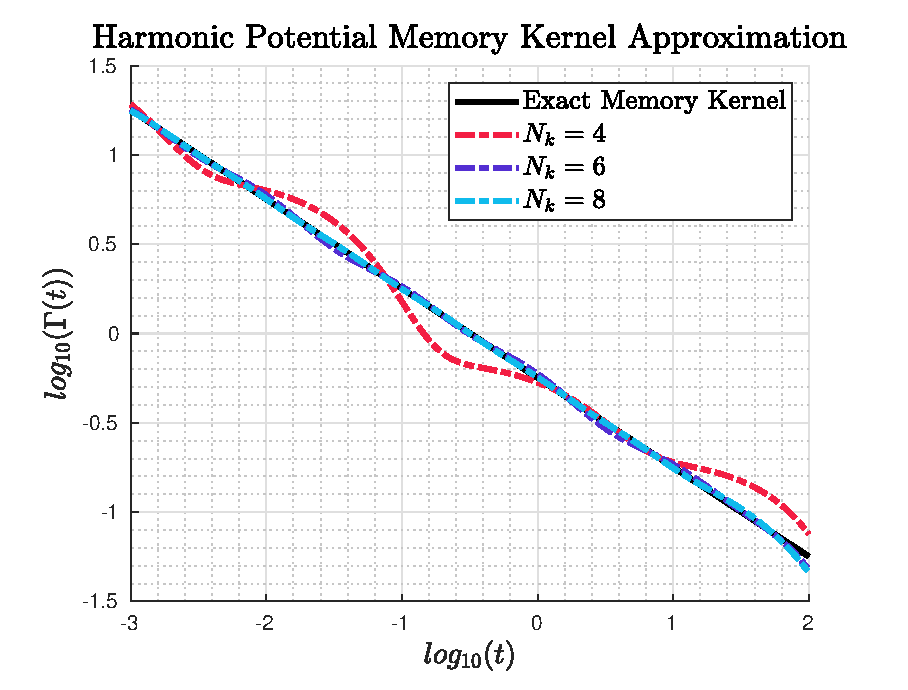
\includegraphics[width=0.75\linewidth]{./Plots/ParameterFittingExample/paramFit.eps}
			\caption{A Prony series fit of the \textit{power law} memory kernel in \cref{eq:HarmonicGLE} for
				$\gamma_{\lambda} = 1$, $\lambda = 0.5$ for different $N_{k}$}
		\end{figure}
	\end{frame}

	\begin{frame}
		\frametitle{\large Harmonic Potential Well - Normalized \texttt{VAF} \& Pointwise Error}
		\footnotesize
		\begin{figure}[H]
			\centering
			\begin{subfigure}[b]{0.48\linewidth}
				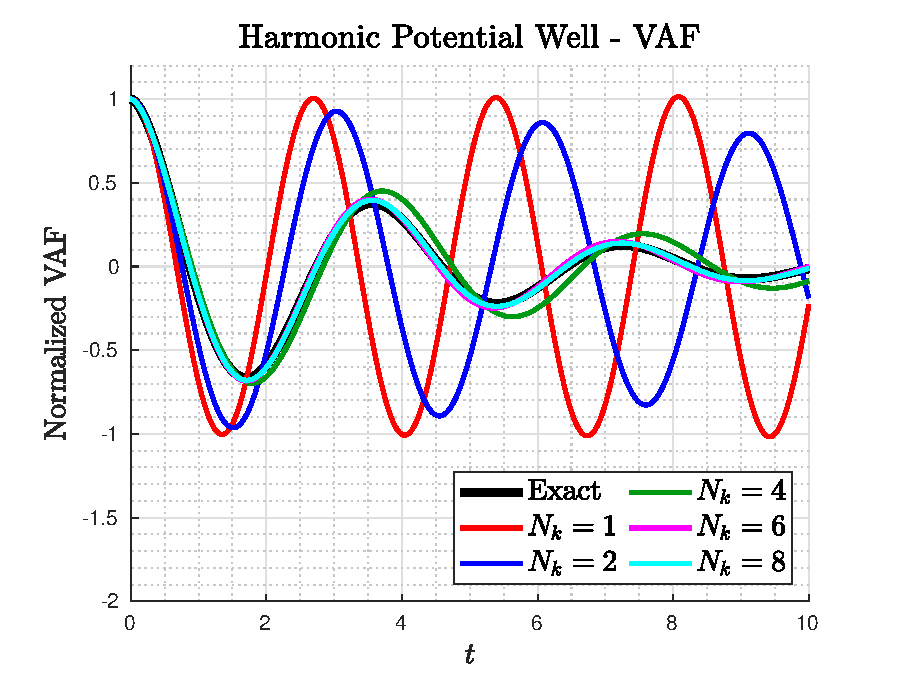
\includegraphics[width=\linewidth]{./Plots/harmonicPotential/solnCompare.eps}
				\caption{\footnotesize Normalized \texttt{VAF} at different times for different no. of modes used in Prony series approximation}
			\end{subfigure}
			\begin{subfigure}[b]{0.48\linewidth}
				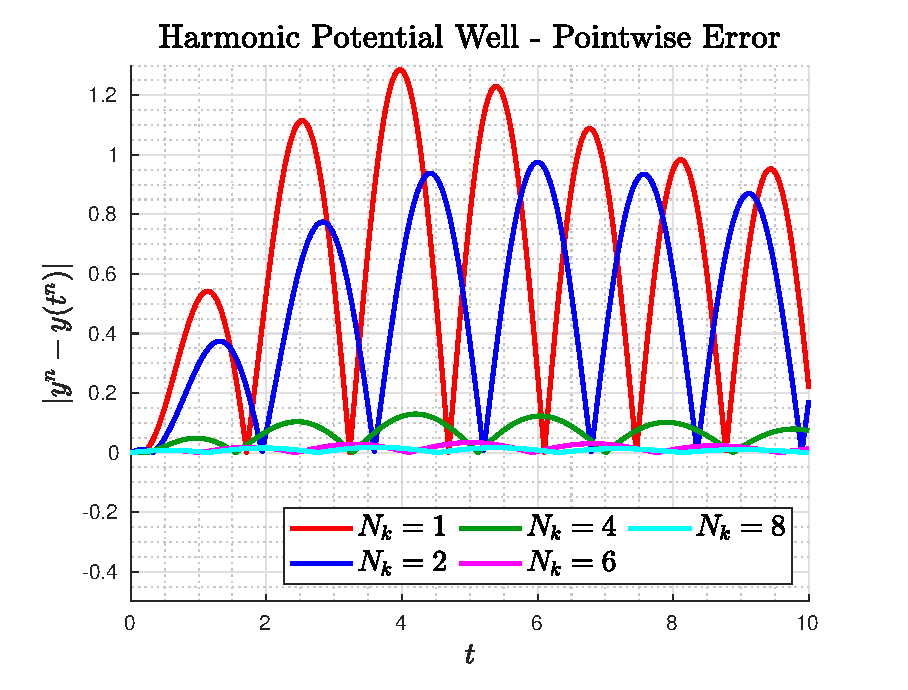
\includegraphics[width=\linewidth]{./Plots/harmonicPotential/errorCompare.eps}
				\caption{\footnotesize Pointwise error in \texttt{VAF} at different times for different no. of modes used in Prony series approximation}
			\end{subfigure}
			\caption{Approximation of the Harmonic Potential Well problem for $\gamma_{\lambda} = 1$, $\lambda = 0.5$ and $\omega_{0} = 1.4$ using Prony series approximation}
		\end{figure}
	\end{frame}

	\begin{frame}
		\frametitle{\large Harmonic Potential Well - Normalized VAF \& Pointwise Error}
		\begin{alertblock}{Normalized \texttt{VAF} - Exact Solution}
			$$ \underbrace{C_{V}(t)}_{\text{Normalized VACF}} = \sum_{k=0}^{\infty} \frac{\rb{-1}^{k}}{k!} \rb{\omega_{0} t}^{2k} \mathscr{E}_{2-\lambda,1+\lambda k}^{(k)}\rb{-\gamma_{\lambda} t^{2-\lambda}}$$
			where $\mathscr{E}_{\alpha,\beta}^{(k)}\rb{y}$ represents the $\text{k}^{\text{th}}$ derivative of the \textit{Generalized Mittag-Leffler} function given by:
			$$ \mathscr{E}_{\alpha,\beta}^{(k)} \rb{y} = \sum_{j=0}^{\infty} \frac{\rb{j+k}! \; y^{j}}{j! \; \Gamma_{0}\rb{\alpha(j+k)+\beta}}$$
		\end{alertblock}
	\end{frame}

	\begin{frame}
		\frametitle{Harmonic Potential Well - Normalized MSD}
		\begin{figure}[H]
			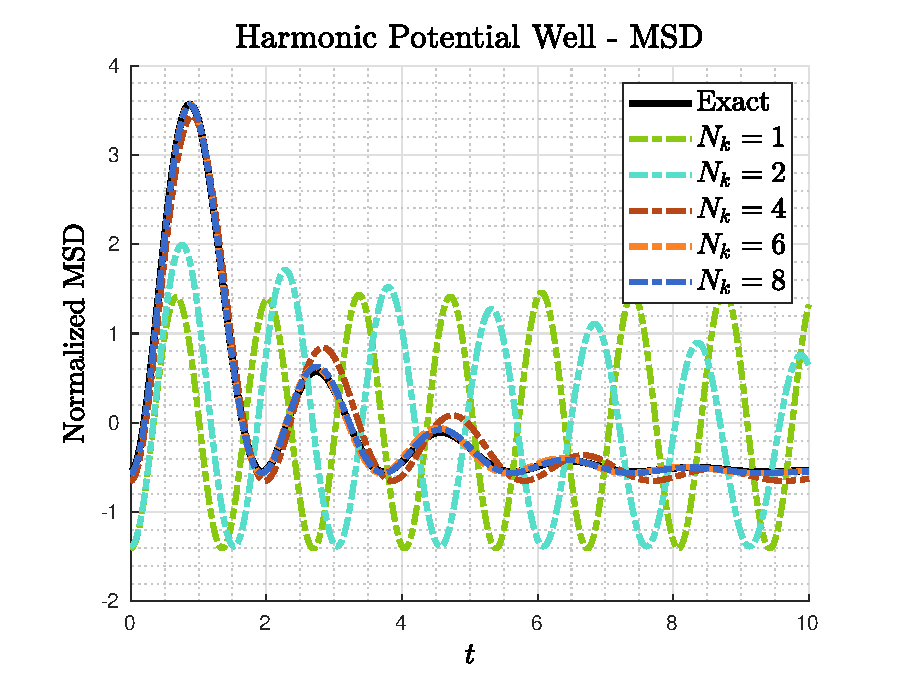
\includegraphics[width=0.725\linewidth]{./Plots/MSD/MSDCompare.eps}
			\caption{Normalized MSD at different times for different no. of modes used in Prony series approximation. ($\gamma_{\lambda} = 1$, $\lambda = 0.5$ and $\omega_{0} = 1.4$)}
		\end{figure}
	\end{frame}
	
	\begin{frame}
		\frametitle{Harmonic Potential Well - Normalized MSD}
		\begin{alertblock}{Normalized \texttt{MSD} - Exact Solution}
			\footnotesize
			\begin{align}
				\notag
				\underbrace{\angbrac{\sqb{\BS{X}(t+\tau)-\BS{X}(t)}^{2}}}_{\text{Normalized MSD}} &= \frac{2\text{k}_{\text{B}}T}{m} I(\tau) - 2 x_{0} v_{0} \omega_{0}^{2} \sqb{G(t+\tau) - G(t)}\sqb{I(t+\tau) - I(t)} \\
				\notag 
				&+ \rb{v_{0}^{2} - \frac{\text{k}_{\text{B}}T}{m}} \sqb{G(t+\tau)-G(t)}^{2} \\
				\notag
				&+ \omega_{0}^{2} \rb{x_{0}^{2} \omega_{0}^{2} - \frac{\text{k}_\text{B} T}{m}} \sqb{I(t+\tau)-I(t)}^{2}
			\end{align}
			\begin{align}
				\notag
				I(t) &= \sum_{k=0}^{\infty} \frac{\rb{-1}^{k}}{k!} \omega_{0}^{2k} t^{2(k+1)} \mathscr{E}^{(k)}_{2-\lambda,3+\lambda k} \rb{- \gamma_{\lambda} t^{2-\lambda}} && \text{(Kernel integral)}\\
				\notag
				G(t) &= \sum_{k=0}^{\infty} \frac{\rb{-1}^{k}}{k!} \omega_{0}^{2k} t^{2k+1} \mathscr{E}^{k}_{2-\lambda,2+\lambda k} \rb{- \gamma_{\lambda} t^{2-\lambda}} && \text{(Relaxation function)}
			\end{align}
		\end{alertblock}
		where $v_{0}$,$x_{0}$ represent the velocity and position of the particles at time $t=0$.
	\end{frame}

	\begin{frame}
		\frametitle{Harmonic Potential Well - Normalized PAF}
		\begin{figure}[H]
			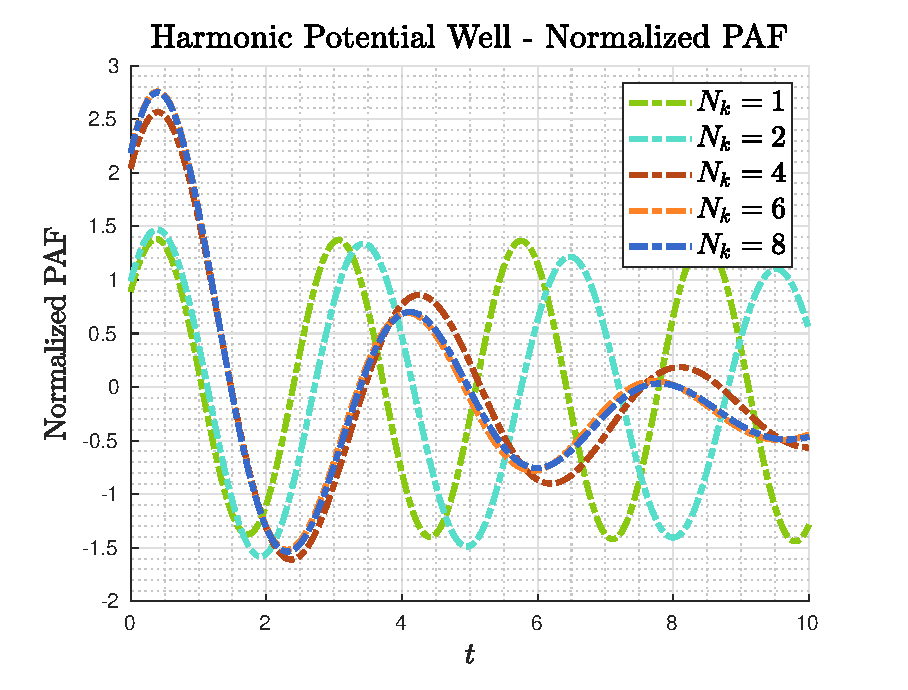
\includegraphics[width=0.75\linewidth]{./Plots/normalizedPAFPlots/normPAF.eps}
			\caption{Normalized PAF, $ \frac{\angbrac{\BS{X}(t),\BS{X}(0)}}{\angbrac{\BS{X}(0),\BS{X}(0)}}$ vs. Time for Harmonic Potential Well problem when approximated with varying no. of terms in the Prony series approximation ($\gamma_{\lambda} = 1$, $\lambda = 0.5$ and $\omega_{0} = 1.4$)}
		\end{figure}
	\end{frame}

	\begin{frame}
		\section{Global and Local Sensitivity Analysis}
		\subsection{Need for Sensitivity Analysis}
		\frametitle{Need for Sensitivity Analysis}
		\textcolor{blue}{\textbf{Question?}} \\ \vspace{0.2cm} Why do we need to perform global and local sensitivity analysis? \vspace{0.2cm} \\
		\textcolor{blue}{\textbf{Answer:}} \\
		\begin{itemize}
			\item {Extended variable GLE fitted by matching \texttt{MSD} or \texttt{VAF} obtained from experimental data. Prony series parameters $c_{k},\tau_{k},N_{k}$ sensitive to experimental data i.e. to errors in measurement or lack of data. Also determine $N_{k}$ such that the error in the fit is lower than certain tolerance.}
			\item {\textit{Ergodicity breaking:} Time averaged statistics such as \texttt{MSD} do not converge to ensemble averages i.e. there is a large "spread" (variance) in the observables.}
		\end{itemize}
	\end{frame}

	\begin{frame}
		\subsection{Local Sensitivity Analysis}
		\frametitle{Mathematical Tools for Local Sensitivity Analysis}
		\begin{block}{Sensitivity Analysis}
			Let $\mathcal{S}\rb{t,\theta;f}$ denote the sensitivity of the stochastic process $\BS{X}_{t}\rb{\theta}$ where $\theta$ is a parameter that affects the stochastic process and $f$ is the given observable. We are interested in calculating:
			$$ \mathcal{S}\rb{t,\theta;f} = \frac{\partial \E{f\rb{\BS{X}_{t}\rb{\theta}}}}{\partial \theta}$$
		\end{block}
		\textcolor{blue}{\textbf{Methods of Calculation:}}
		\begin{itemize}
			\item {\textit{{Finite Difference Stencils:}} Approximating derivative by a finite difference stencil and obtain the required moments by Monte Carlo.}
			\item {\textit{{Likelihood Ratio:}} Expressing sensitivity as an expectation of $f$ under a change of measure.}
			\item {\textit{{Malliavin Calculus:}} Extension of calculus of variations to stochastic processes.}
		\end{itemize}
	\end{frame}
	
	\begin{frame}
		\subsection{Tools available for performing local sensitivity analysis}
		\frametitle{Mathematical Tools for Local Sensitivity Analysis}
			\footnotesize
			\boxed{\texttt{Finite Difference Stencil}}
			$$ \mathcal{S}_{\varepsilon}\rb{t,\theta;f} = \frac{\E{f\rb{\BS{X}_{t}\rb{\theta + \varepsilon}}} - \E{f\rb{\BS{X}_{t}\rb{\theta}}}}{\varepsilon} $$
			\boxed{\texttt{Likelihood Estimator}}
			\begin{align*}
				\mathcal{S}_{LR}\rb{t,\theta;f} = \frac{\partial \E{f\rb{\BS{X}_{t}\rb{\theta}}}}{\partial \theta} &= \int f\rb{x_{t}} \sqb{\partial_{\theta} \log g\rb{\theta,x_{t}}} g\rb{\theta,x_{t}} dx_{t} \\
				\, &= \E{f\rb{\BS{X}_{t}\rb{\theta}} \partial_{\theta} \log g \rb{\theta,\BS{X}_{t}}}
			\end{align*}
			where $g$ represents the change in measure by a p.d.f. \textcolor{red}{$g$ is unknown which means that it is difficult to calculate local sensitivity using likelihood estimator. Also there is no appropriate change of measure on path space as the parameters $c_{k}$ and $\tau_{k}$ appear in both drift and diffusion terms.} \\
			\vspace{0.2cm}
			\boxed{\texttt{Malliavin Calculus}}
			\begin{align*}
				\mathcal{S}_{M}\rb{t,\theta;f} = \E{f\rb{\BS{X}_{T}}h\rb{\cb{\BS{X}_{s}}_{0 \leq s \leq T}}}
			\end{align*}
			where $h\rb{.}$ represents the Malliavin weights that are non-unique. \textcolor{red}{$h(.)$ is difficult to calculate as it involves solving a system of auxiliary processes obtained using Malliavin Calculus.} 
	\end{frame}

	\begin{frame}
		\subsection{Efficient Local Sensitivity Analysis using FD stencils and Coupled Random Path}
		\frametitle{\large Efficient Local Sensitivity Analysis using FD Stencils for Coupled Random Path}
		\footnotesize
		\textcolor{blue}{\textbf{Objective:}} To find a reduced variance sampling strategy for calculating the local sensitivity.\\
		\vspace{0.15cm}
		\textcolor{blue}{\textbf{Methodology:}}
		Let $\hat{\phi}\rb{\theta}$ represent the expected value of the observable $f\rb{\BS{X}_{t}\rb{\theta}}$. Then we can write,
		\footnotesize
		\begin{align*}
			\hat{\phi}\rb{\theta} = M^{-1} \sum_{i=1}^{M} f\rb{X_{i,t}\rb{\theta}} \Rightarrow \mathcal{S}_{\varepsilon} \rb{t,\theta;\hat{\phi}} \approx \Delta_{c} \rb{M,\varepsilon} = \frac{\hat{\phi}\rb{\theta + \varepsilon}-\hat{\phi}\rb{\theta-\varepsilon}}{2\varepsilon} \\
		\end{align*}
		%\normalsize
		where each random variable is sampled independently of each other.
		\footnotesize
		\begin{align*}
			\Rightarrow \text{Var}\sqb{\Delta_{c}} &= \varepsilon^{-2} \text{Var} \sqb{\hat{\phi} \rb{\theta + \varepsilon} - \hat{\phi} \rb{\theta - \varepsilon}} \\ &= \varepsilon^{-2} M^{-1} \text{Var} \sqb{\underbrace{f\rb{\BS{X}_{t}\rb{\theta + \varepsilon}}}_{R_{1}} - \underbrace{f\rb{\BS{X}_{t}\rb{\theta - \varepsilon}}}_{R_{2}}}
		\end{align*}
		%\normalsize
		where the variance can be rewritten as
		\footnotesize
		$$ \text{Var}\sqb{\Delta_{c}} = \varepsilon^{-2} M^{-1} \rb{\text{Var}\sqb{R_{1}} + \text{Var}\sqb{R_{2}} - 2 \text{Cov} \sqb{R_{1},R_{2}}} $$ 
	\end{frame}
	
	\begin{frame}
		\frametitle{\large Efficient Local Sensitivity Analysis using FD Stencils for Coupled Random Path}
		\textit{Statistical Error} is given by $\epsilon_{M} = \frac{C_{\alpha} \sigma}{\sqrt{M}}$ where $\sigma = \sqrt{\text{Var}\sqb{\Delta_{c}}}$ and $C_{\alpha}$ is a constant based on the confidence level of the solution \\
		\vspace{0.15cm}
		\textcolor{blue}{\textbf{Coupled vs. Decoupled Noise:}}
		\begin{itemize}
			\item {If $R_{1}$ and $R_{2}$ are not correlated, then $\text{Var}\sqb{\Delta_{c}} = \mathcal{O}\rb{\varepsilon^{-2} M^{-1}}$}
			\item {If $R_{1}$ and $R_{2}$ are positively correlated, then $\text{Var}\sqb{\Delta_{c}} = \mathcal{O}\rb{M^{-1}}$}
		\end{itemize}
		\textcolor{blue}{\textbf{Observation:}} \\
		Let $\varepsilon = 0.1$. In order to reduce the error by a factor of $10$.
		\begin{itemize}
			\item {\textit{Coupled Noise:} $M = 10^{2}$ samples}
			\item {\textit{Decoupled Noise:} $M = 10^{4}$ samples}
		\end{itemize}
		Hence the statistical error becomes independent of the perturbation parameter on using a common random path coupling i.e. $R_{1}$ and $R_{2}$ use the same Wiener process $dW$.
	\end{frame}

	\begin{frame}
		\subsection{Results for Global and Local Sensitivity Analysis}
		\frametitle{Local Sensitivity Analysis - Coupled vs. Decoupled Random Path}
		\begin{figure}[H]
			\begin{subfigure}[b]{0.48\linewidth}
				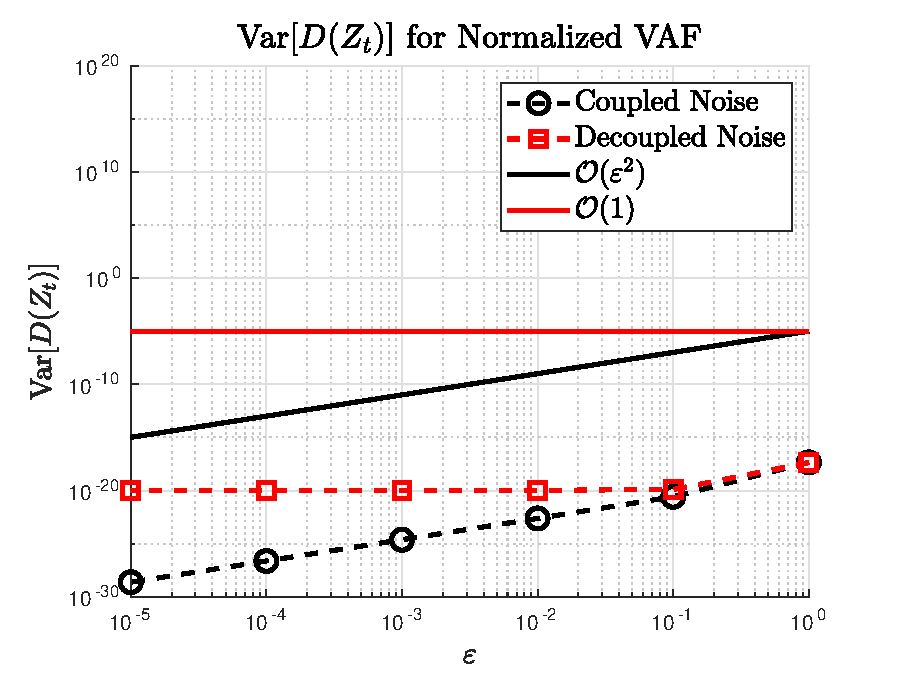
\includegraphics[width=\linewidth]{./Plots/sensitivityAnalysis/VarianceC1.eps}
				\caption{\scriptsize $\text{Var}\sqb{D\rb{Z_{t}}}$ for Normalized VAF where $D\rb{Z_{t}} = \rb{\hat{f}\rb{\theta + \varepsilon} - \hat{f}\rb{\theta - \varepsilon}}$}
			\end{subfigure}
			\begin{subfigure}[b]{0.48\linewidth}
				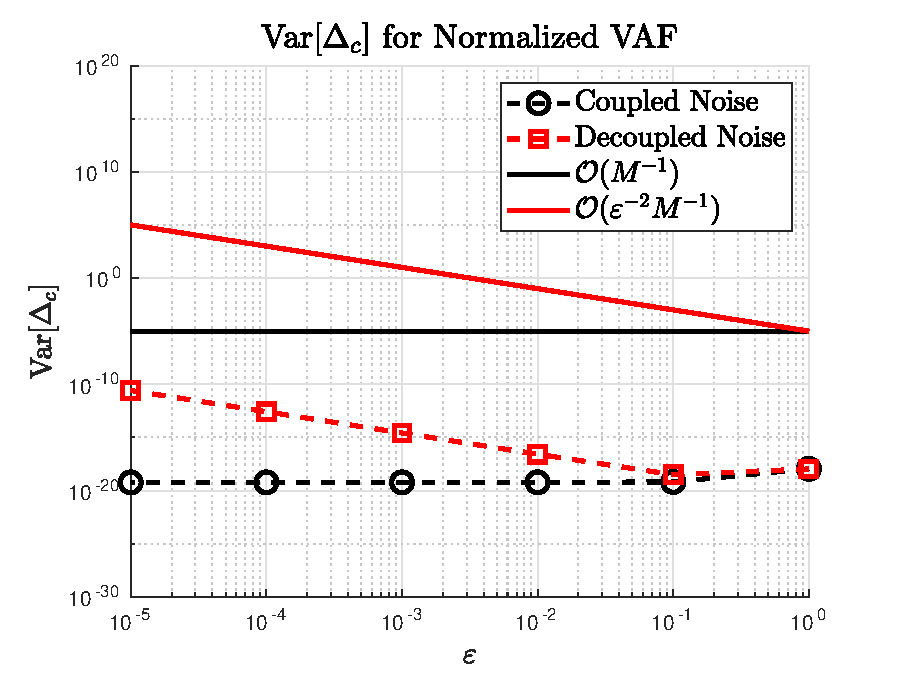
\includegraphics[width=\linewidth]{./Plots/sensitivityAnalysis/VarianceC1_CD.eps}
				\caption{\scriptsize $\text{Var}\sqb{\Delta_{c}}$ for Normalized VAF where $\Delta_{c} = \rb{\hat{\phi}\rb{\theta+\varepsilon} - \hat{\phi}\rb{\theta-\varepsilon}}/2\varepsilon$}
			\end{subfigure}
		\caption{Order of variance reduction when using \textit{Coupled} vs. \textit{Decoupled} noise term on perturbing $c_{1}$. ($M=200,\delta t = 0.1,N_{p} = 1000$) }
		\end{figure}
	\end{frame}

	\begin{frame}
		\frametitle{Local Sensitivity Analysis - Parameter Perturbation}
		\begin{figure}[H]
			\centering
			\begin{subfigure}{0.32\linewidth}
				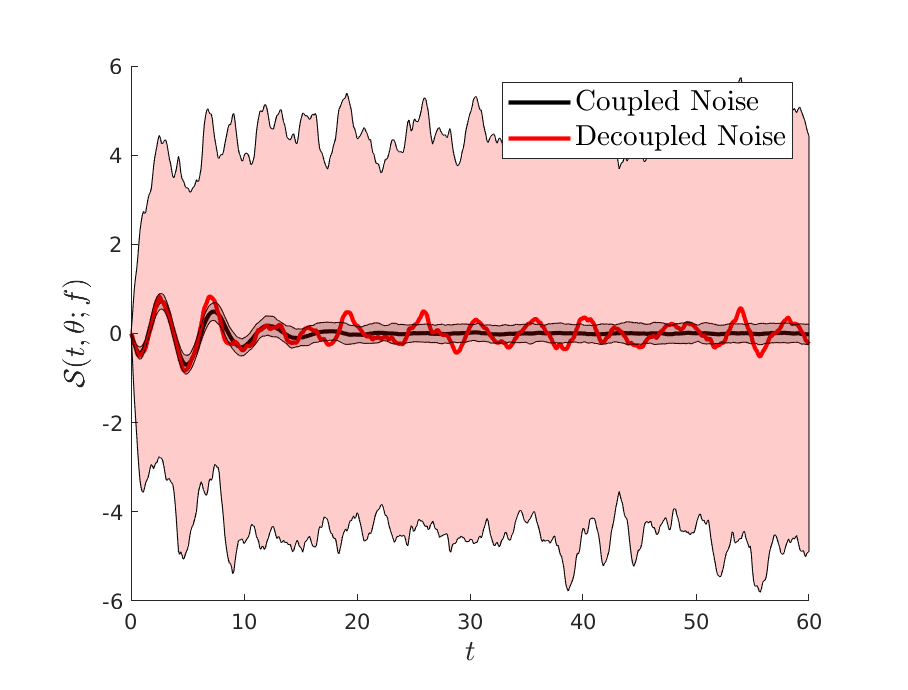
\includegraphics[width=\linewidth]{./Plots/sensitivityAnalysis/c1M100.eps}
				\caption{\tiny $\mathcal{S}_{\varepsilon} \rb{t,c_{1};\text{VAF}}, M = 10^{2}$}
			\end{subfigure}
			\begin{subfigure}{0.32\linewidth}
				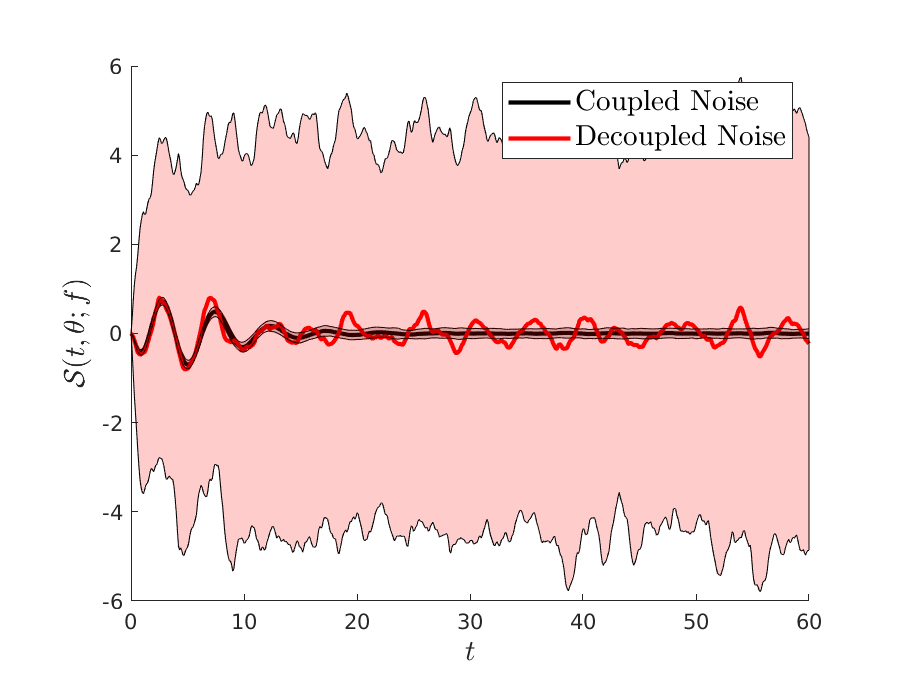
\includegraphics[width=\linewidth]{./Plots/sensitivityAnalysis/c3M100.eps}
				\caption{\tiny $\mathcal{S}_{\varepsilon} \rb{t,c_{3};\text{VAF}}, M = 10^{2}$}
			\end{subfigure}
			\begin{subfigure}{0.32\linewidth}
				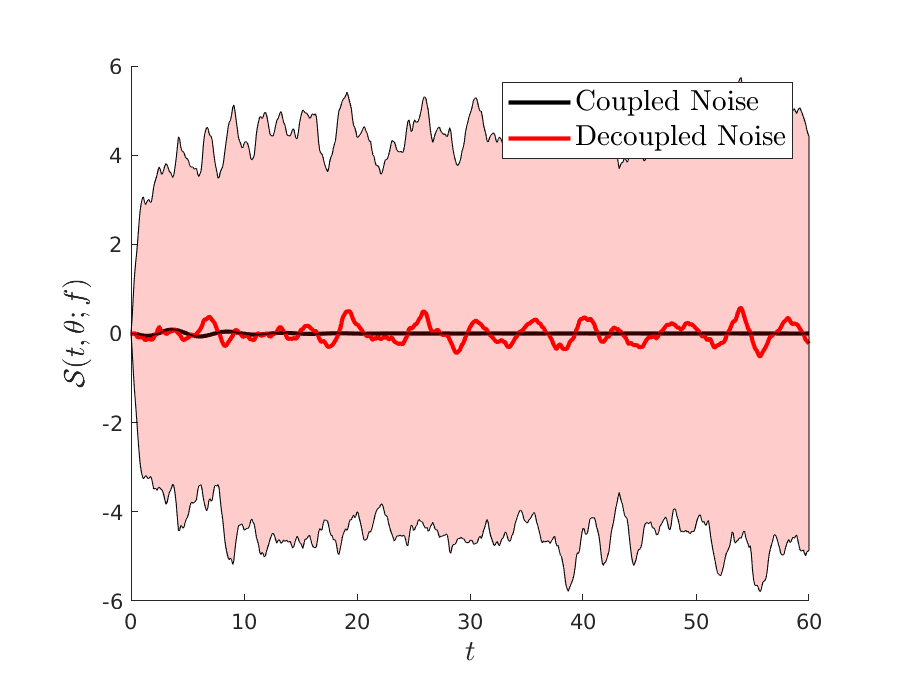
\includegraphics[width=\linewidth]{./Plots/sensitivityAnalysis/c6M100.eps}
				\caption{\tiny $\mathcal{S}_{\varepsilon} \rb{t,c_{6};\text{VAF}}, M = 10^{2}$}
			\end{subfigure}
			\begin{subfigure}{0.32\linewidth}
				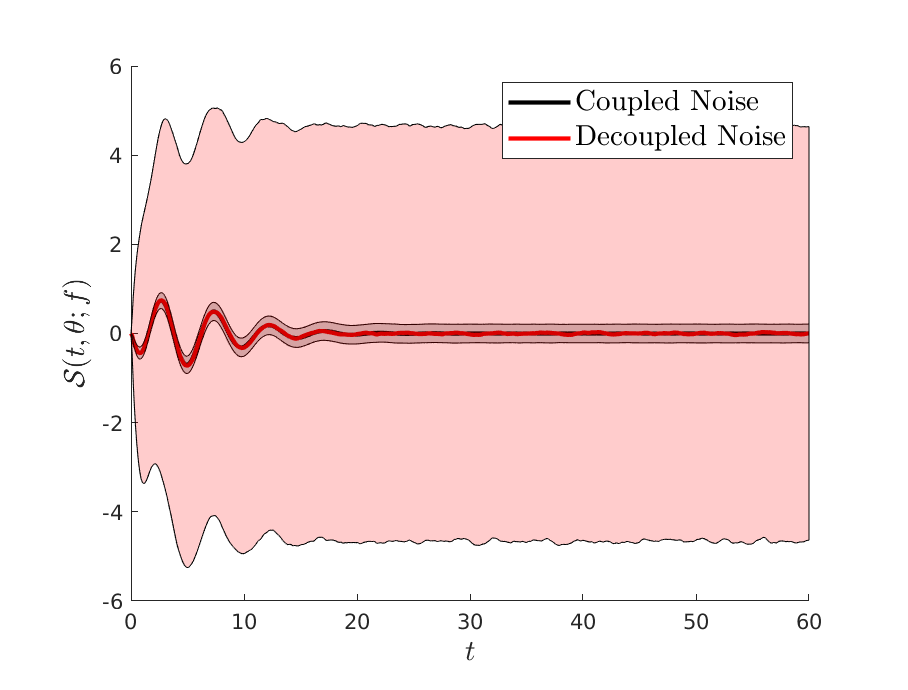
\includegraphics[width=\linewidth]{./Plots/sensitivityAnalysis/c1M10000.eps}
				\caption{\tiny $\mathcal{S}_{\varepsilon} \rb{t,c_{1};\text{VAF}}, M = 10^{4}$}
			\end{subfigure}
			\begin{subfigure}{0.32\linewidth}
				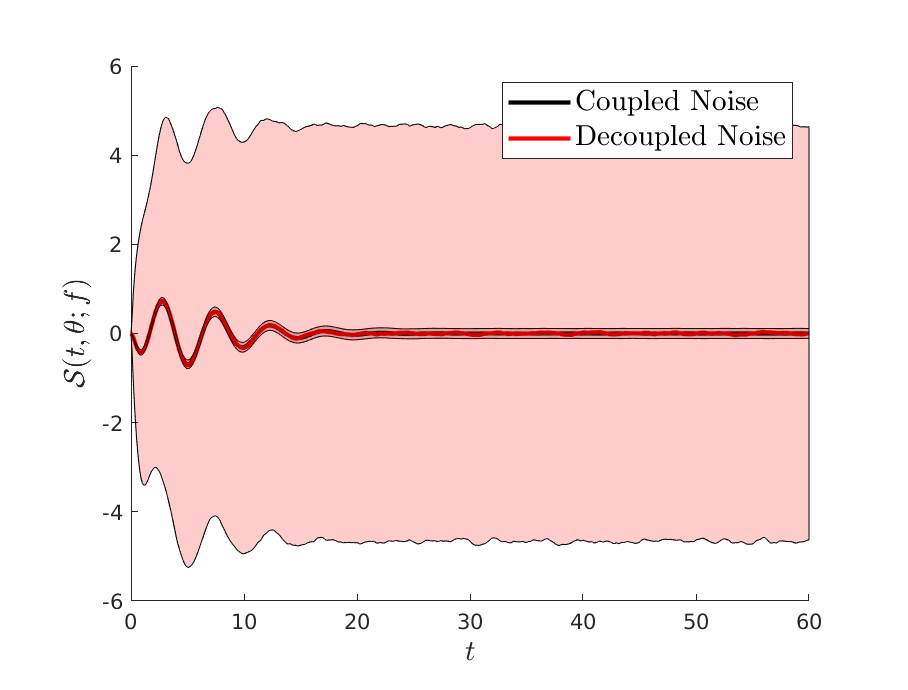
\includegraphics[width=\linewidth]{./Plots/sensitivityAnalysis/c3M10000.eps}
				\caption{\tiny $\mathcal{S}_{\varepsilon} \rb{t,c_{3};\text{VAF}}, M = 10^{4}$}
			\end{subfigure}
			\begin{subfigure}{0.32\linewidth}
				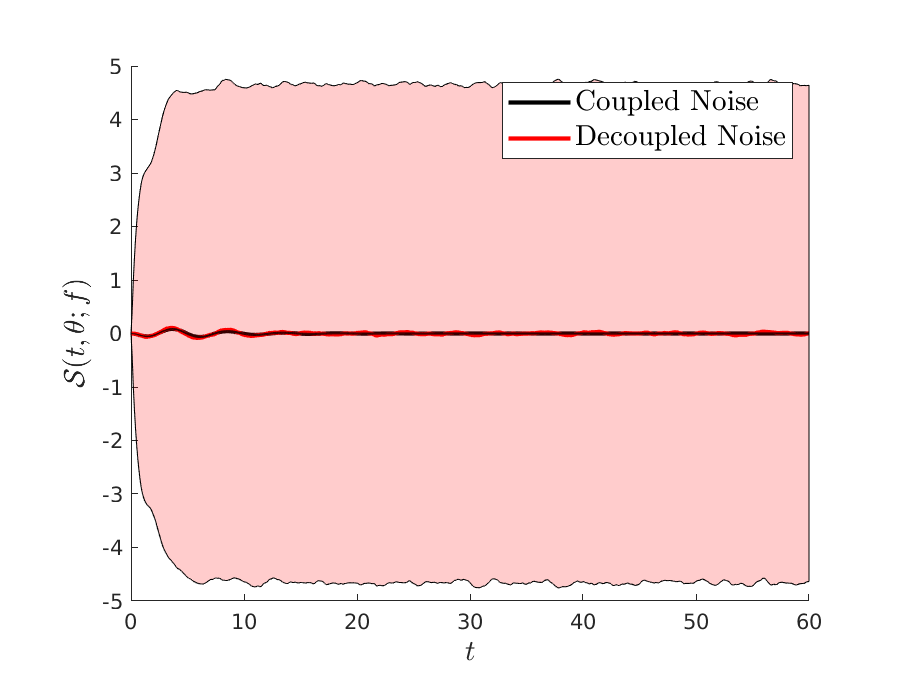
\includegraphics[width=\linewidth]{./Plots/sensitivityAnalysis/c6M10000.eps}
				\caption{\tiny $\mathcal{S}_{\varepsilon} \rb{t,c_{6};\text{VAF}}, M = 10^{4}$}
			\end{subfigure}
			\caption{Local sensitivity of observable, VAF, due to perturbation of $c$ $\rb{\varepsilon = 0.01, \omega_{0} = \frac{8}{9}, \text{k}_{\text{B}} T = 10^{-5}}$}
		\end{figure}
	\end{frame}

	\begin{frame}
		\frametitle{\large Global Sensitivity Analysis - No. of Modes Perturbation}
		\begin{figure}[H]
			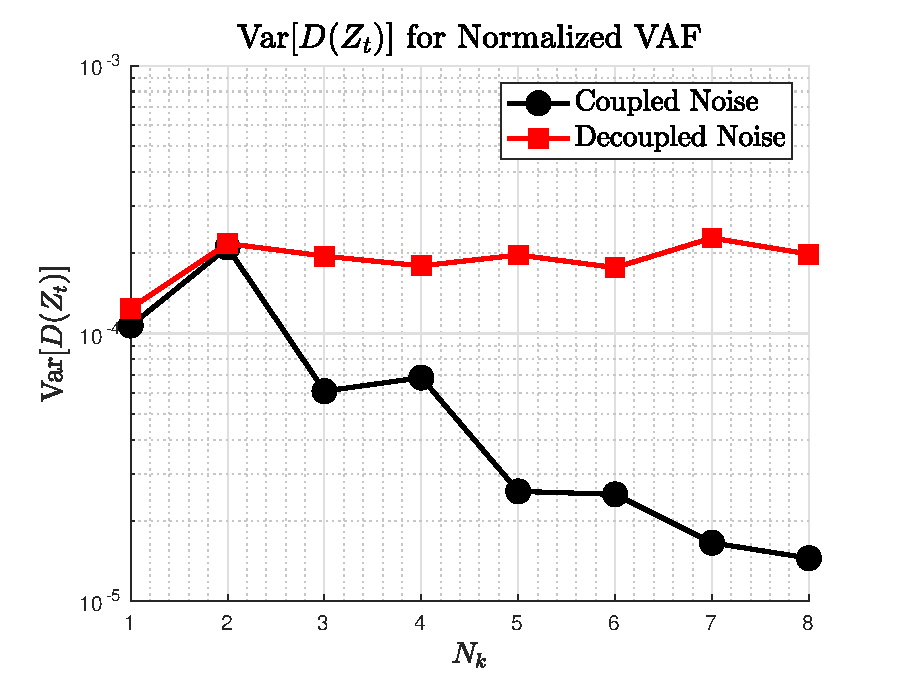
\includegraphics[width=0.5\linewidth]{./Plots/sensitivityAnalysis/NkSensitivity.eps}
			\caption{\footnotesize Var$\sqb{D\rb{Z_{t}}}$ where the difference in solution, $D\rb{Z_{t}}$, is between the nominal model with $N_{k} = n$ and the perturbed model with $N_{k} = n+1$ where $n = 1, \cdots, 8$ ($\omega_{0} = 8/9,\text{k}_{\text{B}}T = 10^{-5},t=100$).}
		\end{figure}
		Though this does not provide a measure for local sensitivity, this provides us information for deciding when we have enough no. of modes in the Prony series approximation of Extended Variable GLE system i.e. the system is no longer sensitive to capture more memory.
	\end{frame}

	\begin{frame}
		\frametitle{\large Global Sensitivity Analysis - No. of Modes Perturbation}
		\begin{figure}[H]
			\centering
			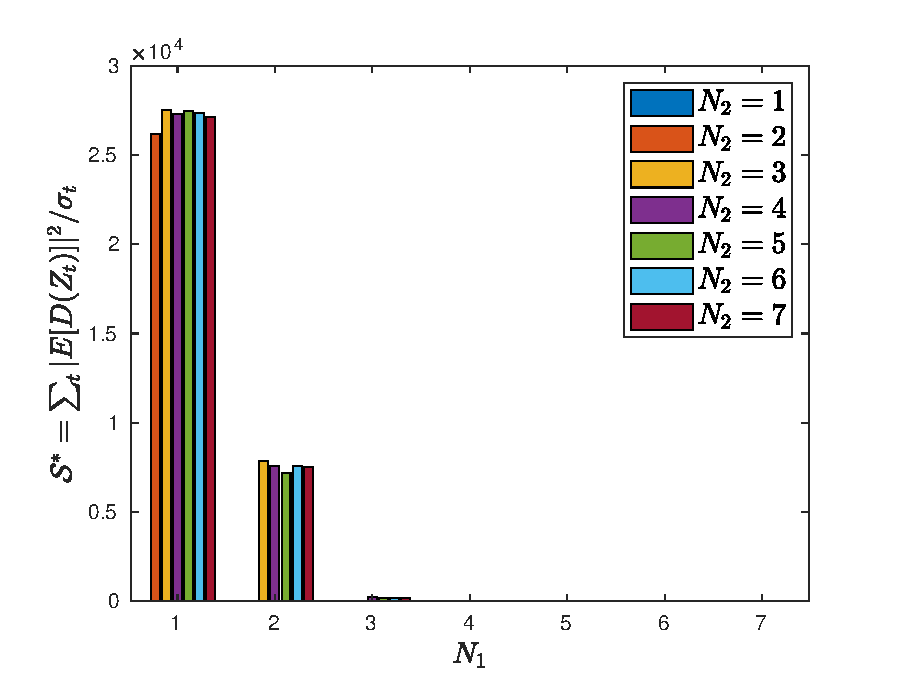
\includegraphics[width=0.75\linewidth]{./Plots/sensitivityAnalysis/SStarCoupled.eps}
			\caption{The global sensitivity index $\mathcal{S}^{*} = \sum_{t} \left| \E{D\rb{Z_{t}}} \right| ^{2} / \sigma_{Z_{t}}$ gives a quantitative characterization of the difference between the observed VAF on varying the no. of Prony series modes. ($\omega_{0} = 8/9,\text{k}_{\text{B}}T = 10^{-5},t=50,M=10^{2}$).}
		\end{figure}
	\end{frame}

	\begin{frame}
		\section{Conclusion}
		\frametitle{Conclusion}
		%\footnotesize
		\textcolor{blue}{\textbf{Extended Variable GLE:}}
		\begin{itemize}
			\item {\textit{Non-Markovian} challenge overcome by converting to \textit{Markovian} extended variable GLE problem using Prony series approximation.}
			\item {Explicit Euler scheme does not conserve $1^{\text{st}}$ and $2^{\text{nd}}$ moments unlike Splitting scheme.}
			\item {Number of modes used in Prony series approximation affects the \texttt{memory kernel} fit.}
		\end{itemize}
		\textcolor{blue}{\textbf{Sensitivity Analysis:}}
		\begin{itemize}
			%\item {Sensitivity analysis was performed using \texttt{Central Difference} finite difference stencil}
			\item {Significant reduction in variance of the calculated sensitivity on using a common coupled random path for the diffusion term of GLE.}
			\item {Order of variance reduction for $D\rb{Z_{t}}$ was observed to be $\mathcal{O}\rb{\varepsilon^{2}}$ for coupled noise and $\mathcal{O}\rb{1}$ for decoupled noise.}
			\item {Order of variance reduction for $\Delta_{c}$ was observed to be $\mathcal{O}\rb{M^{-1}}$ for coupled noise and $\mathcal{O}\rb{\varepsilon^{-2}M^{-1}}$ for decoupled noise.}
		\end{itemize}
	\end{frame}

	\begin{frame}
		\section{Outlook}
		\frametitle{Outlook}
		\large
		\begin{itemize}
			\item {Parameter fitting over experimental data to see how the noise in the experimental data affects the model.}
			\item {Compatibility study of Prony series approximations to other complex potentials.}
			\item {Expressing memory kernel in a form such that the problem can be solved using Krylov subspace methods.}
		\end{itemize}
	\end{frame}
		
	\begin{frame}[allowframebreaks]
		\section{References}
		\frametitle{References}
		\footnotesize
		\nocite{Baczewski2013}
		\nocite{Berne1966}
		\nocite{Desposito2009}
		\nocite{Hall2016}
		\nocite{Higham2001}
		\nocite{Kawasaki1973}
		\nocite{Leimkuhler2015}
		\nocite{Lysy2016}
		\nocite{Vinales2006}
		\bibliography{./citations.bib}
	\end{frame}
\end{document}